\chapter{\chapviname}
\label{chapter6}
\textit{The content from this chapter is predominantly from the manuscript published in the proceedings of Electroactive Polymers Actuators and Devices XXVI.}

\begin{center}
\section*{ABSTRACT}
    Dielectric elastomer actuators commonly use flexible conductive electrodes to apply an electric potential to the system. Depending on the material used, these electrodes often possess predictable piezo-resistive properties. Combining electrical impedance tomography (EIT) with a dielectric elastomer actuator (DEA) is investigated in this work to map compressive forces occurring throughout the electrode surfaces. This technology could allow for enhanced closed-loop control of electroactive actuators, extending their already extensive set of applications. This deformation mapping system also has the potential to be used with other piezoresistive materials, opening up more applications requiring a large hardness range and pressure sensitivity. With the material used in this work, the DEA-EIT device has an inherent trade-off between actuation and pressure mapping accuracy driven by the compliant electrode thickness of the DEA. The DEA-EIT device exhibited actuation strains of 2.5 \% with a mean centre-of-mass error from a range of loads applied were 7.9 $\pm$ 0.7 mm for 2 mm thick DEA electrodes. It is proposed that future work on custom hardware could be devised for the DEA-EIT system so the sensing and actuation can occur concurrently in real-time. Real-time control mean that applications requiring human-like manipulation can be designed, ranging from biomedical implant devices to agricultural processing equipment. 	
\end{center}

	
\section{INTRODUCTION} % 1.5 pages
	\label{sec:introduction}
     Fine motor manipulation, pressure sensitivity, and pressure mapping are some core attributes of skin and muscle tissues when innervated to the brain. These functions can be emulated and combined with two core technologies, Dielectric Elastomer Actuators (DEAs), and Electrical Impedance Tomography (EIT) based pressure mapping.
	
	DEAs have been used to mimic biological muscles in many applications, because of the technology's likeness to biological muscle in terms of elasticity, energy density, and various potential shapes/topologies \cite{Rosset2016, Hajiesmaili2021, Guo2021} . In previous research, it was determined that pressure mapping similar to that of human mechanoreceptors could be emulated using EIT with a piezoresistive nanoparticle elastomer composite (PNEC) in a planar sheet format\cite{Ellingham2022} . The key qualities of the EIT-based sensing platform were that pressure estimates could be obtained, the pressure could be mapped, and the spatial performance could be quantified\cite{Ellingham2024} . Like DEAs, this sensing technology has a likeness to human tissue in terms of mechanical characteristics such as elasticity, and the potential of various topologies.
	
	Alongside the visual and other sensory feedback, animals receive when actuating muscle tissue, pressure-sensitive mechanoreceptors are present within the muscle tissue and soft skin tissue to aid control the extent of a muscle contraction. This forms a multi-sensor closed-loop control system with a complex biological control regime. This work is looking towards creating a closed-loop control system which utilises a DEA-based artificial muscle and an EIT-based artificial skin.
	
	
	\subsection{Background} 
	\label{subsec:background}
	% Add any other original background about DEAs and EIT, and potential failure modes
	The fundamental principles and a brief explanation of the state-of-the-art of each DEA and EIT-based sensor technologies are given in this section. A review of pressure mapping devices with actuation capabilities was then completed. At the time of completing this work, no literature had been found regarding the combination of these two technologies using PNEC electrodes on a DEA for successive execution of sensing and actuation events.  
	
	\subsubsection{Dielectric Elastomer Actuators}
	\label{subsubsec:deas}
	DEAs are often referred to as artificial muscles because they share similar characteristics to biological muscle. DEAs have been proven to produce strains larger than 1600 \%\cite{Keplinger2012} which is significantly larger than that of regular biological muscle. However, large DEA strains can often be at the cost of actuator instability and a low effective force. DEAs have a high work and power density comparable to that of biological muscle and have been found experimentally to have energy densities of around 3.4 J.g$^{-1}$ and theoretically an order of magnitude more\cite{Liu2009, Koh2009} . A dielectric elastomer actuator (DEA) is a form of soft robotic actuator that induces deformation with an applied electric field. Although commonly used as an actuator, this technology offers versatile applications as an energy generator\cite{McKnight2002, Carpi2008, Koh2009} or sensor and provides attractive features such as high energy density, large displacements, and fast response times. A simple configuration of a DEA is a circular parallel plate capacitor, which consists of a thin elastomer sheet between two compliant conductive electrodes, as shown in Figure \ref{fig:DEA_diagram}. When a voltage is applied to the compliant electrodes, the electrostatic force arises between the electrodes causing the dielectric elastomer (DE) membrane to contract by a decrease in thickness and an increase in area. The resulting actuation is controlled by changing the applied voltage. The region encompassing the two compliant electrodes and the DE portion sandwiched between them is called the `active region'. For a simple DEA such as the one shown in Figure \ref{fig:DEA_diagram}, a simplified formula for the electrode static force on the parallel plates is given in Equation \ref{eqn:DEA_stress}.
	\begin{equation}
		\sigma_{es} = \varepsilon_0 \varepsilon_r \frac{V^2}{z_{de}^2}
		\label{eqn:DEA_stress}
	\end{equation}
	Where $\sigma_{es}$ is the electrostatic stress, $V$ is the applied voltage, $z_{de}$ is the DE thickness, $\varepsilon_0$ is the permittivity of free space, and $\varepsilon_r$ is the relative permittivity constant of the DE, which is a function of strain\cite{Kofod2003, Choi2005, Wissler2007} and applied voltage\cite{Rosset2013} . This can be expanded to include the bulk modulus, $K$, of the DE as given in Equation \ref{eqn:DEA_strain_z}.
	\begin{equation}
		S_{z_{de}} = \frac{\sigma_{es}}{K}
		\label{eqn:DEA_strain_z}
	\end{equation}
	\begin{figure}[H]
		\centering
		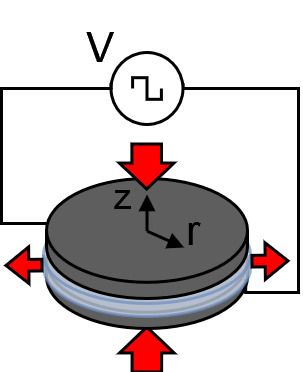
\includegraphics[width=5cm]{Figures/circ_DEA_v2.jpg} % TODO: add cylindrical coords and 'V' for voltage source
        \vspace{0.2cm}
		\caption{A circular DEA exemplifying its actuation principle.}
		\label{fig:DEA_diagram}
	\end{figure}
	
	\subsubsection{Soft EIT-based Pressure Mapping}
	\label{subsubsec:eit-based_pressure_mapping}
	% Discuss: state of the art, our previous work
	A soft EIT-based pressure mapping sensor has the ability to estimate the magnitude and location of force loads in a planar PNEC material. The hardware required usually consists of a piezoresistive sensor domain with attached boundary electrodes, EIT driver electronics, and a reconstruction processor. Boundary electrodes allow a non-invasive method of pressure mapping without compromising a monolithic piezoresistive material. Several researchers have created an EIT-based pressure mapping sensor using a range of piezoresistive domains and custom or lab-based hardware \cite{Russo2017, Nagakubo2007, Silvera-Tawil2015, Yoon2017, Sun2020, Ellingham2024}.
	
    EIT devices can perform at image frame rates higher than 50 Hz, however using EIT to map and quantify piezoresistive pressure events has the potential to give a faster sample rate due to the use of DC instead of AC. Due to the viscoelastic and resistive nature of the sensor, the frequency response can be lower than that of the frame rate of the sensor depending on the piezoresistive sensing domain used. 
 
    The stages required to generate a pressure image using EIT can be simplified into three core stages,
	\begin{enumerate}
		\item Data acquisition
		\item Image reconstruction
		\item Inverse pressure model
	\end{enumerate} 
	\begin{figure}[H]
		\centering
		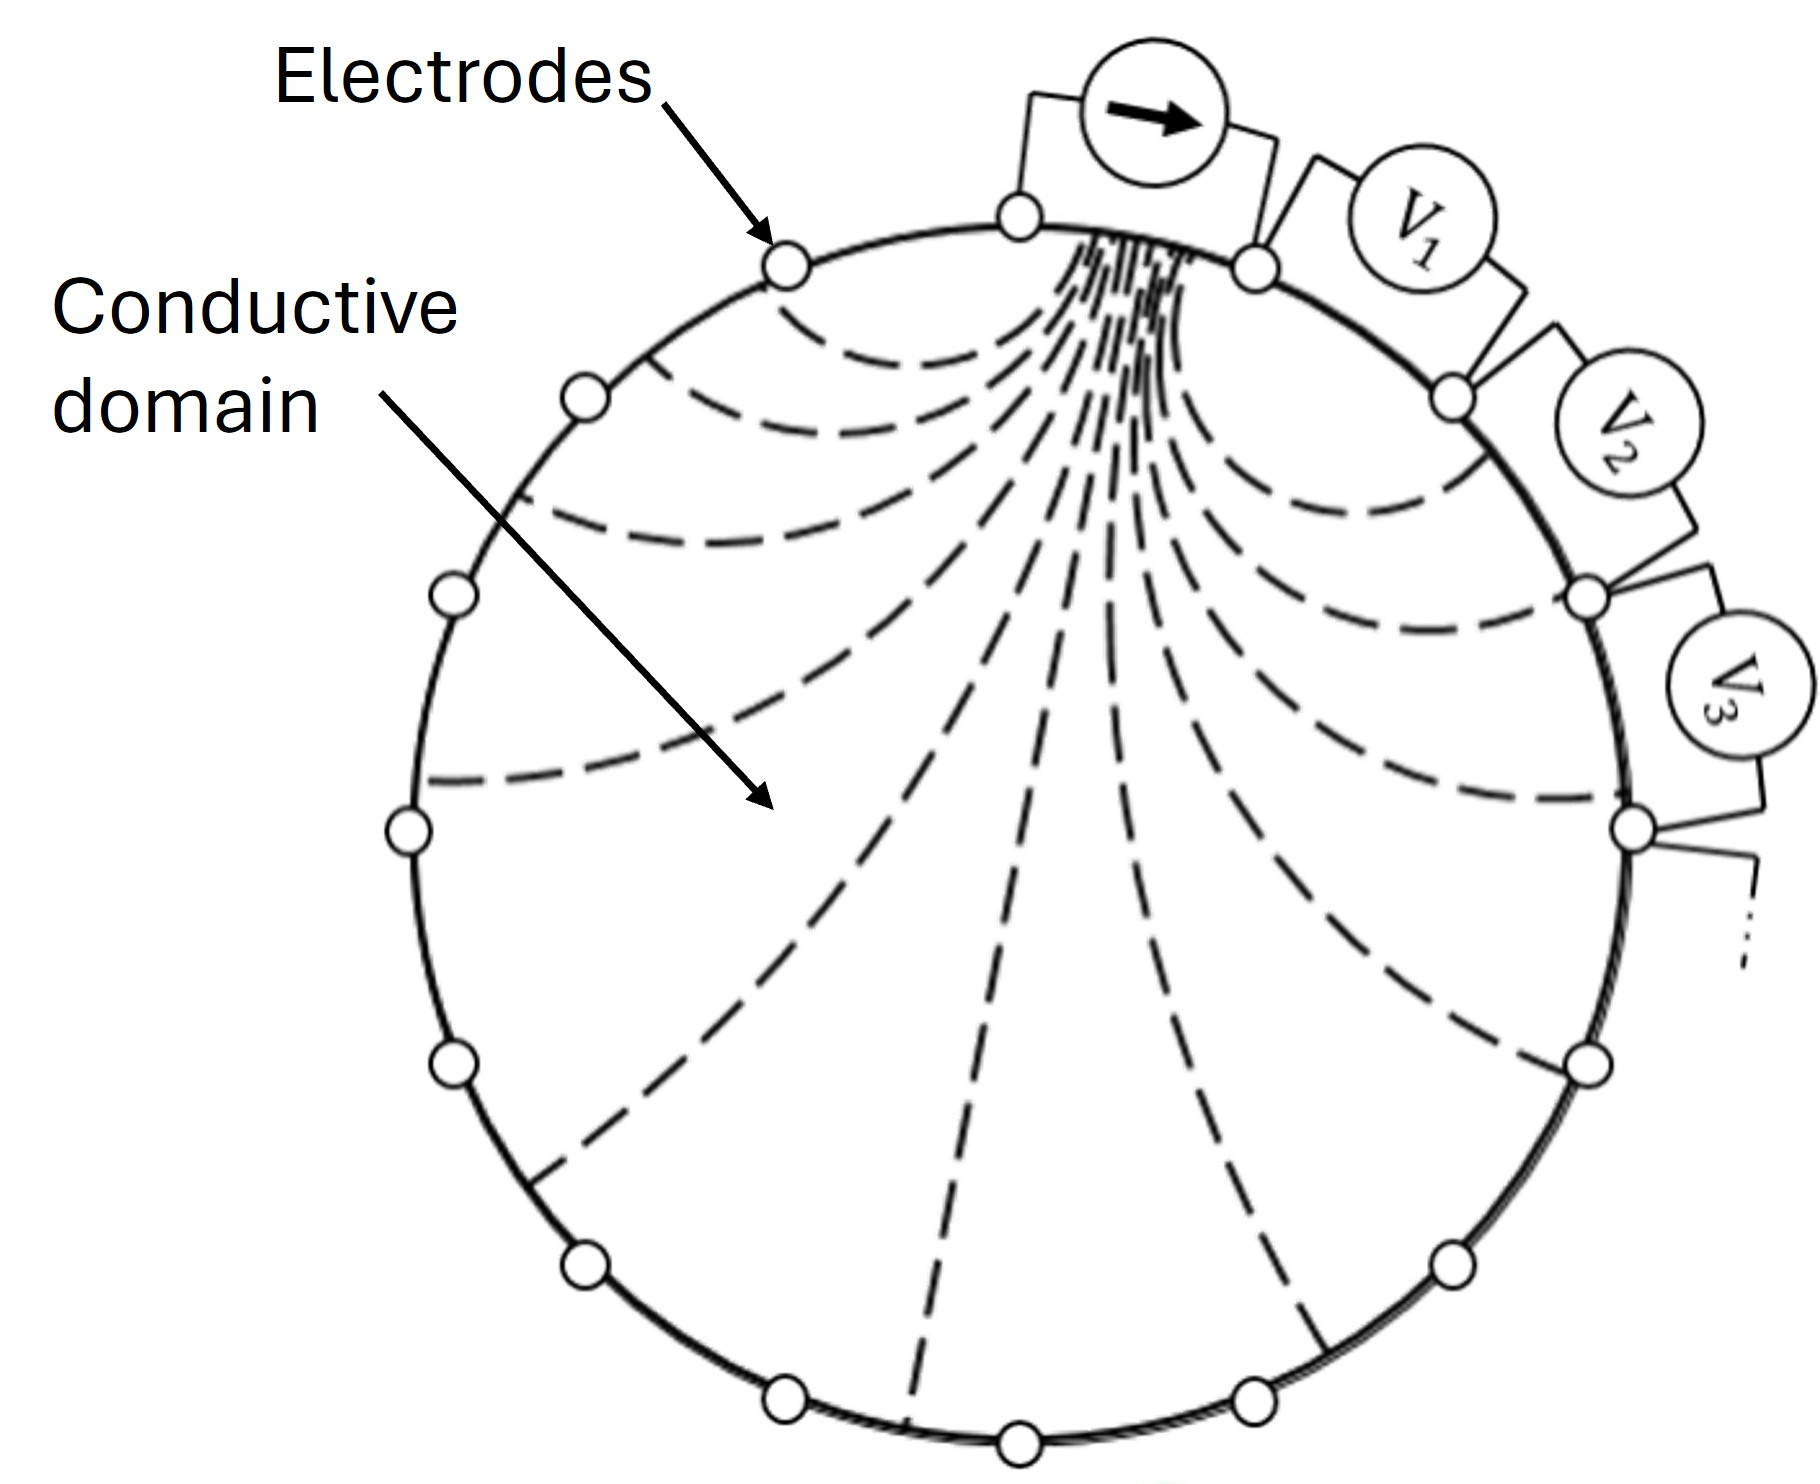
\includegraphics[width=5cm]{Figures/EIT_diagram_labelled.jpg}
        \vspace{0.2cm}
		\caption{A 16 electrode circular EIT domain setup exemplifying its electrical function. Where the dashed lines are representative of an applied electric field\cite{Ellingham2022} .}
		\label{fig:EIT_diagram}
	\end{figure}
	Data acquisition involves an excitation drive pattern to be applied to the piezoresistive sensing domain, which consists of the injection of a known current or voltage through two boundary electrodes connected to the material domain as shown in Figure \ref{fig:EIT_diagram}. Typically an adjacent electrode drive pattern is used in literature as it is used in this work\cite{Russo2017} . Concurrently all voltages at the other boundary electrodes of the material domain are read. Then the known current (or voltage) source is applied to the next set of adjacent electrodes, and all of the other adjacent electrode voltages are read once more. This process is repeated until it has been deemed there have been sufficient readings to solve the inverse problem and generate a conductance, $\rho$, distribution estimate of the material domain. Finally, an inverse model converting the conductance estimate of the material domain can be converted into a pressure map using an inverse model.
	
	
	\subsection{Simultaneous Pressure Mapping and Actuation}
	\label{subsec:sensing_and_actuation}
	Various researchers have demonstrated and proposed the use of self-sensing DEAs for closed-loop control looking at the one-dimensional deformation of a DEA using capacitance\cite{Gisby2013, Liu2016, Huang2023, Koshiya2023} . Multi-degree-of-freedom (multi-DOF) DEA topologies have been created by several researchers \cite{Nguyen2017, Zhang2024, Zou2023, Pei2004}, allowing for a broader range of applications. The complex actuation mechanisms discussed in these papers give rise to the question of having more resolute sensor data for such topologies to aid with the control of such multi-DOF devices.

    To ensure the DEA maintains minimal change to the parallel plate topology, the compliant piezoresistive electrodes can be used and/or altered to be able to determine the deformation of the DEA in more than one dimension using EIT. EIT-based DEA sensing offers several potential advantages over other methods of pressure sensing, such as the use of boundary electrodes, using existing compliant electrode material as sensing domains, simple drive circuitry, and various sensing domain shapes.
	
	% To sense deformation in multiple dimensions, the current methods used for DEA self-sensing must be altered. To ensure the DEA maintains minimal change to the parallel plate topology, the compliant piezoresistive electrodes can be used and/or altered to be able to determine the deformation of the DEA in more than one dimension. Options for sensing in two dimensions include determining the stretch across the compliant electrode material by measuring the change in resistance of the electrodes diametrically opposed at various angles around the DEA, or adding an extra pressure mapping sensor layer to the DEA stack, or using EIT to map change in resistance of the compliant electrodes. Using diametrically opposed resistance measurements across the compliant electrodes will have limited resolution and is limited in compliant electrode shapes that can be used effectively. Adding another sensing layer to the DEA requires a sensing technology that has a very low elastic modulus, to not hinder the actuation force of the DEA. The limitations given above are why EIT was chosen to sense 2D deformation of a DEA, as it has a relatively high spatial resolution that can be quantified and requires no extra hardware on the DEA apart from non-invasive electrodes on the boundary of the DEA's compliant electrode(s).
	
	% Add any references here that are very similar/related to our work HERE!
	% e.g. \cite{Deshpande2005}
	
	% Explain some example applications:
	% Gripper object identification - e.g. pick up an object using a DEA gripper identify what it may be and place it in a certain box.
	% A conical DEA that can throw a ball and then sense where it lands so it can then shoot the ball back into the air again. No optics required.
	
	% To localise where a dielectric breakdown has occurred to help for the active healing of the device through another separate technology.
	
	% Create a DEA that uses a kind of beamforming (not super feasible ~18GHz req for creating 10mm wavelengths... fun theory to do though) to create an inhomogeneous strain with the DEA that can react/mimic to a strain compression input in the DEA.
	

 
	\section{METHODOLOGY} % 3 pages
	\label{sec:method}
	The DEA-EIT actuator-sensor-hybrid system required the two technologies to be verified and fabricated individually before being integrated to observe the effects of combining the two technologies relative to their independent forms. The following sections discuss the fabrication process for the DEA and EIT systems and the integration of them both into a DEA-EIT system.
	
	To optimise the actuation and sensing capabilities of the DEA-EIT system different parameters of design were altered, such as the compliant electrode composite, DE, circumferential electrodes, and magnitude of DE pre-stretch and sizing. The methodology explores the reasoning behind certain design choices for the fabrication of the DEA design seen in Figure \ref{fig:DEA_components}.
	
	
	\subsection{Dielectric Elastomer Preparation}
	\label{subsec:de_fab}
	The fabrication of the DEA used a rigid acrylic frame to attach the pre-stretched elastomer. For simplicity, a circular frame was chosen with the DE at a radial pre-stretch of +10\%, i.e. $\lambda_r$ = 1.1, as this is well within the DE's more predictable linear elastic region. The circular acrylic frame of 178 mm inner diameter was fabricated from laser cut acrylic of 4 mm thickness to ensure rigidity.
	
	To achieve uniform stretch of the elastomer sheet, a toroidal shower hose mechanism was placed on the relaxed sheet of 4910 VHB tape (3M, Saint Paul, USA), which would act as a pre-stretcher annulus. The toroidal mechanism has an axis of rotation along its circumference as shown in, giving the ability to roll and stretch the elastomer equiaxially to the desired pre-stretch. 
	\begin{figure}[H]
		\centering
		% \subfloat[Elastomer pre-stretch method]{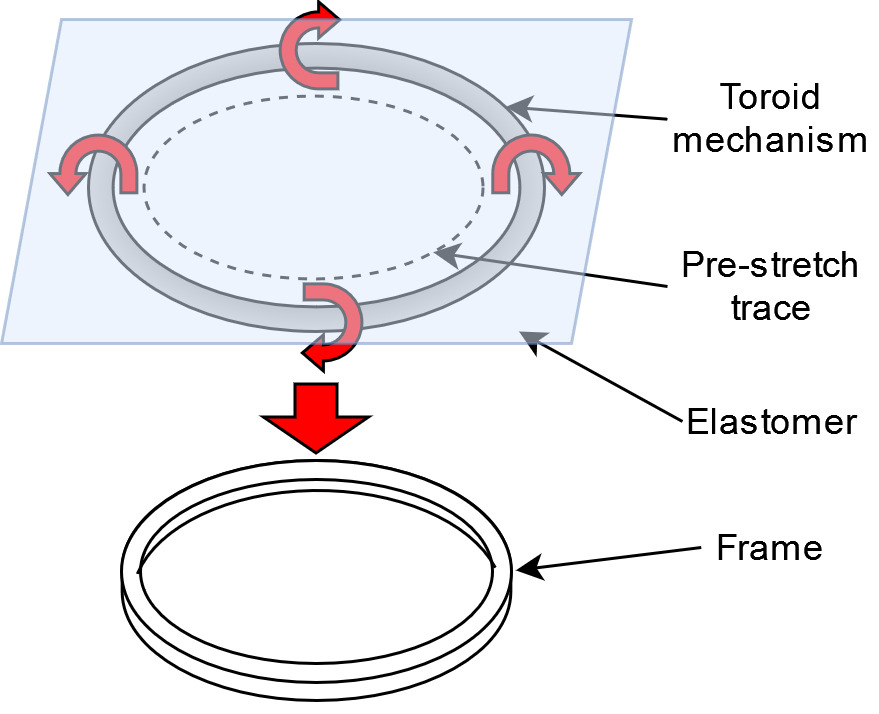
\includegraphics[width=5cm]{Figures/DEA_fab_mech.jpg}\label{subfig:DEA_pre-stretch}}
		% \hspace{0.5cm}
		\subfloat[Circular DEA construction]{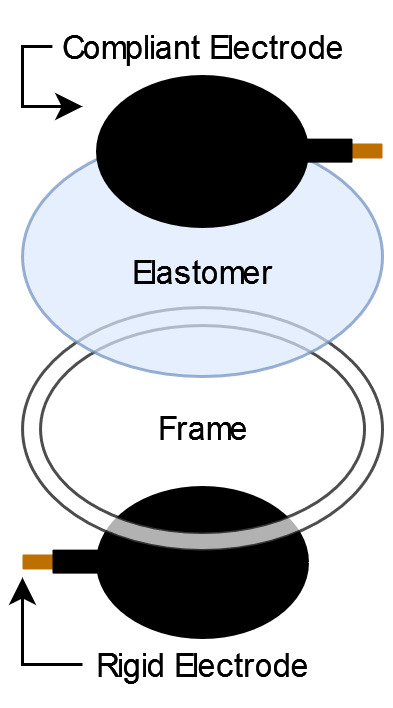
\includegraphics[width=3.5cm]{Figures/DEA_stack.jpg}\label{subfig:DEA_stack}}
		\hspace{1cm}
		\subfloat[Single circumferential electrode]{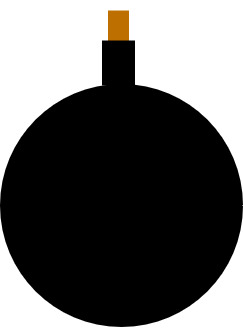
\includegraphics[width=3cm]{Figures/DEA-EIT_single.jpg}\label{subfig:DEA_EIT_single}}
        \hspace{1cm}
		\subfloat[Multiple circumferential electrodes]{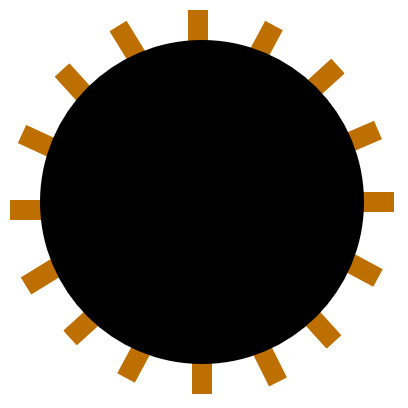
\includegraphics[width=4cm]{Figures/DEA-EIT_multi_elec.jpg}\label{subfig:DEA_EIT_multi}}
		\vspace{0.2cm}
		\caption{Mechanical fabrication of the circular DEA-EIT platforms}
		\label{fig:DEA_components}
	\end{figure}x
	
	
	\subsection{Compliant Electrode Fabrication}
	\label{subsec:dea_elec_fab}
	% TODO: Either remove "75 mm" or complete more EIT testing on the 75 mm electrodes
	Compliant electrodes (or active area) were fabricated using acrylic moulds of varying dimensions. Three thicknesses, $z_{ce}$, of the compliant electrode were fabricated, 0.5 mm, 1 mm and 2 mm, with two circular compliant electrodes of 100 mm diameter. Different thicknesses were explored as this would vary the actuation and sensing performance of the electrodes.
	
	Two compliant electrode mediums were used in this work, carbon black (CB) powder and a carbon black silicone rubber (CBSR) composite. Compliant electrodes solely made of CB powder have been used in DEAs in previous literature\cite{Carpi2015, Huang2022, Shigemune2018} , hence this work uses the same compliant electrode type to generate reference data. The CB powder was used to make a single circumferential electrode configuration DEA as a reference to compare to the following DEA-EIT experiments. The CBSR composite was used to make both single (Figure \ref{subfig:DEA_stack}) and multiple (Figure \ref{subfig:DEA_EIT_multi}) circumferential electrode configurations of DEAs. The CB powder used in all of the compliant electrode samples was Vulcan XC-72 powder (Fuel Cell Store, Bryan, USA). The CBSR composite had 8\% CB by weight mixed with DragonSkin 10NV silicone rubber (Smooth-On, Macungie, USA). This composite is a piezoresistive medium that has proven useful for EIT pressure mapping and sensing in previous work\cite{Ellingham2024} , and DEA actuation\cite{Carpi2015, Huang2022} .
	
	Using the liquid silicone rubber, the CBSR composite mixture was formed by combining part A of the silicone solution and 8 wt\% CB and mixing by hand for 10 s. The mixture was then placed in the ARV-310PCE planetary vacuum mixer (Thinky Inc., Tokyo, Japan) to complete a mixing cycle with 500 RPM for 45 s followed by a cycle with 800 RPM for 45 s. In the same mixing container, part B of the silicone solution was added to the mixture and stirred by hand for 10 s and immediately the same mixing cycle in the planetary mixer was completed again. After the cycle was completed, the composite was poured into the mould with attached circumferential copper tape electrodes. The CBSR mixture was then placed in an oven at 80 $\degree$C for 4.5 h to ensure the composite was sufficiently cross-linked.
	
	Two types of compliant electrode configuration have been fabricated in this work, single circumferential electrode and multiple circumferential electrodes. The single circumferential electrode configuration was purely for testing the DEA actuation. The multiple circumferential electrode configuration consisted of 16 evenly spaced circumferential electrodes. The multiple circumferential electrode configuration was for testing both pressure mapping and actuation functionality of the DEA. Prior to curing the compliant electrode in a circular mold, the conductive copper tape circumferential electrodes were placed into the mold. The width of the circumferential electrodes was 8 mm. The circumferential electrodes were placed with a 3 x 8 mm area embedded in the compliant electrode circumference edge with the rest of the circumferential electrode protruding for easy access to external electrical connections.
	% \begin{figure}[H]
		%     \centering
		%     \includegraphics[width = 0.6\textwidth]{Figures/1st_batch_cropped.jpg}
		%     \caption{2mm thick silicone-based carbon black composite}
		%     \label{fig:label}
		% \end{figure}
	
	
	\subsection{DEA Hardware}
	\label{subsec:dea_hw}
	The excitation voltage for the DEA was provided by a Trek 610E high voltage supply (Advanced Energy Industries, Fort Collins, USA) providing a maximum voltage output of 10 kV DC. The DEA was placed in a clear insulated box with the high voltage supply leads attached to the rigid copper electrodes of the DEA. An iPhone 11 camera (Apple Inc., Cupertino, USA) was used to obtain images of the radial compliant electrode strain as shown in Figure \ref{fig:HV_DEA_setup}. The current limit of the high voltage supply was set to its maximum of 2 mA to ensure the DEA actuation was not limited by the charging of the compliant electrodes.
	\begin{figure}[H]
		\centering
		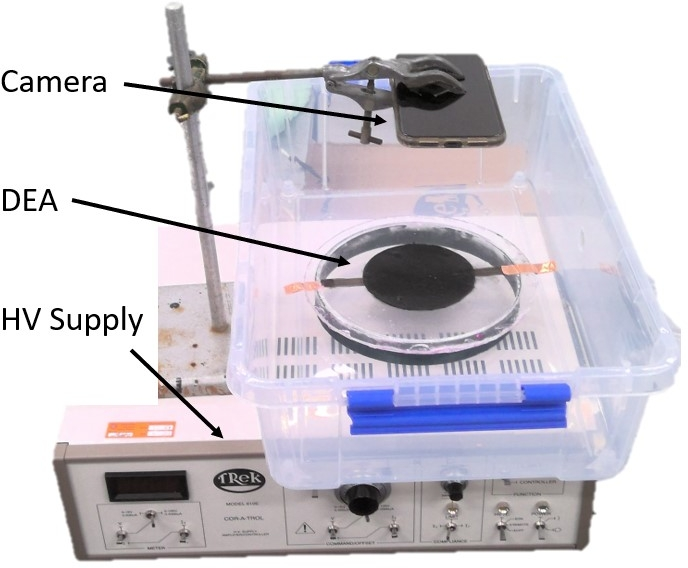
\includegraphics[width=8cm]{Figures/HV_DEA_setup_labelled.jpg}
        \vspace{0.2cm}
		\caption{DEA excitation and measurement setup}
		\label{fig:HV_DEA_setup}
	\end{figure}
	
	
	\subsection{EIT Hardware}
	\label{subsec:eit_hw}
	The EIT hardware allows for data collection to reconstruct a conductance map of the of piezoresistive composite used as compliant electrodes in the DEAs. The hardware required for this function, shown diagrammatically in Figure \ref{fig:ERT_MUX_CFA}, includes a 2634b source measure unit (SMU) (Keithley, Solon, USA), a custom 4:16 multiplexer (MUX) PCB, an ESP32 development board, a Cartesian force applicator, and a reconstruction and control computer. 
	\begin{figure}[H]
		\centering
		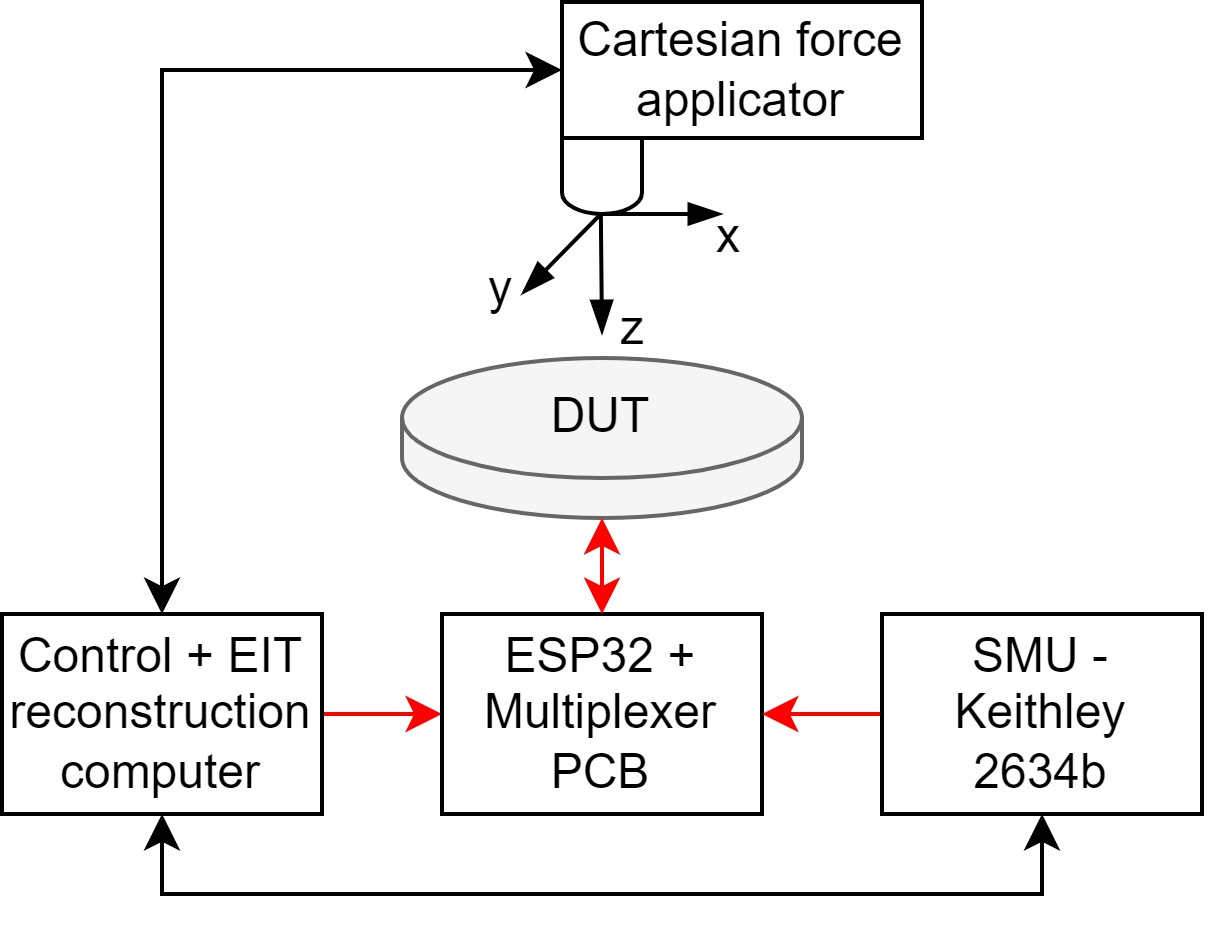
\includegraphics[width=8cm]{Figures/ERT_MUX_CFA_architecture.jpg}
        \vspace{0.2cm}
		\caption{Architecture of the force applicator and EIT measurement system \cite{Ellingham2024}}
		\label{fig:ERT_MUX_CFA}
	\end{figure}
	The SMU provides a constant current value of 1 mA and reads a series of voltages through the MUX PCB required for the EIT drive pattern. An adjacent electrode EIT drive pattern was used for EIT through the circumferential electrodes of the compliant electrode. The MUX PCB and SMU and controlled by the control computer. Once the data for each image reconstruction has been gathered the control computer was also used for the reconstruction of the conductivity maps of the compliant electrodes. The Cartesian force applicator is made up of a MK3s 3D printer (Prusa, Prague, Czechia) integrated with a loadcell and fabricated applicator tip to apply loads and hence generate data for pressure magnitude and localisation quantification.
	
	
	\subsection{Experimental Method}
	\label{subsec:experimental_method}
	Before attempting to have simultaneous DEA actuation and EIT sensing occur in the same device, each system had to be tested independently. First DEA strain voltage relationships were explored, followed by EIT-based pressure mapping of the DEA electrodes. Finally, the same samples used for EIT testing were subsequently integrated into a DEA device for actuation testing.
	
	\subsubsection{DEA Validation} % TODO?: move DEA bits below EIT stuff to show the intended sequence of operations/experiments 
	\label{subsubsec:dea_validation1}
	DEA actuation strain measurements were taken from voltages 5 kV to 10 kV in 1 kV increments. The SNR of strain measurements of the DEA excited with voltages $<$ 5 kV were deemed to be too low to generate meaningful data. The excitation voltage was toggled between on and off states waiting for the strain deflection to reach a steady state for the strain measurements. Five radial strain images were captured and measured. The measurements were then averaged to minimise error and determine the radial strain uniformity. The radial strain was found by measuring the radial change of the circular compliant electrodes between relaxed and electrically contracted states. From the radial compliant electrode strain the planar and thickness deformation of the DE was estimated. The DE is assumed to be incompressible and have a Poisson's ratio, $\nu$, of 0.5. The adhesion between the compliant electrode and the DE is assumed to be perfect to simplify the model used here. The thickness strain, $S_{z_{de}}$, is calculated using Equations \ref{eqn:DEA_strain_z_r}\cite{Carpi2015} and \ref{eqn:DEA_stress}.
	% The experimental data was collected using a series of photographs of the DEA capturing the radial strain of the compliant electrodes. The radial strain of each steady state image of an excitation state was averaged over 5 measurements, to minimise measurement error and observe any non-uniform radial deformation.
	\begin{equation}
		S_{z_{de}} = \frac{1}{(S_{r_{ce}} + 1)^2} - 1
		\label{eqn:DEA_strain_z_r}
	\end{equation}
	Where $S_r$ is the radial strain measured from the equi-biaxial actuation. 
	The elastic modulus of a hyperelastic material such as VHB is often defined as a non-linear function of strain and strain rate\cite{Liu2018} . In this work a bulk modulus value, $K$, of 142 kPA was used. The bulk modulus was determined by doing a meta-analysis and averaging of the elastic moduli determined at steady state 10\% strain for VHB 4905 material in previous literature\cite{Liu2018, Helal2018, Huang2023} .
	% VHB mechanical modulus in lit :::
	% Liu2018 Y @ 10% strain: Y(static) = 178 kPa, Y(dyn) = 225 kPa, tensile?? Y = 290 kPa
	% Helal2018 Y split into a kelvin-voight model? : Ys = 130 kPa(elastic modulus), Yp = 242 kPa(elastic component of loss), Dp = 1.958 MPa (loss modulus)
	% Huang2023 Y @ 10% strain : Y = 119 kPa
	The relative permittivity, $\varepsilon_r$, used in Equation \ref{eqn:DEA_stress} was approximated to be 4.5$\pm$0.2 due to pre-strain effects seen in literature\cite{Kofod2003, Choi2005, Wissler2007, Pan2015} .
	% VHB rel permittivity in lit :::
	% Askounis2020 : e_r = 4.2 (no strain mentioned)
	% McKay2009 : e_r = 4.5 (zero strain), 4.6 - 6 (for a range of electric field strengths applied??) -- only abstract available..
	% Kofod2003 : 4.7 in unstretched state. 4.45 in stretched state.
	% TODO: mention how these assumptions will add to the error seen in the data and how other works have made models not requiring such assumptions! Here or in discussion??
	% TODO: Mention how the compliant electrode K_eff will be a non-linear function of thickness, d. This function is very important for determining half of the objective function to optimise for actuation AND sensing. 
	\begin{figure}[H]
		\centering
		\subfloat[The reference DEA made with CB powder compliant electrodes]{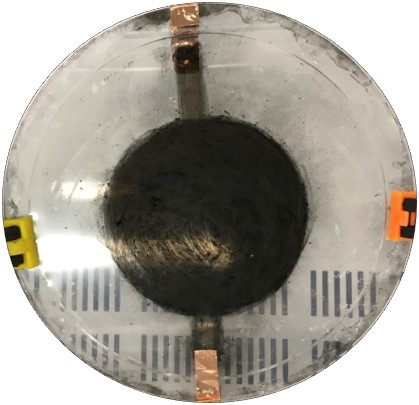
\includegraphics[width = 6cm]{Figures/CB_DEA_crop.jpg}\label{subfig:ref_DEA}}
		\hspace{1cm}
		\subfloat[A DEA with 0.5 mm thick compliant electrodes at steady state contraction and excited at 10 kV.]{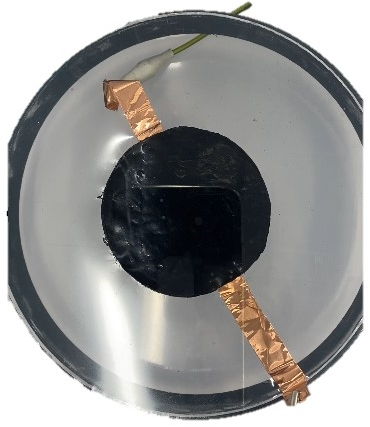
\includegraphics[width = 5.6cm]{Figures/10kV_0.5mm_75mm_CBSR_RMBG.jpg}\label{subfig:CBSR_DEA_10kV}}
        \vspace{0.2cm}
		\caption{Two main types of DEA compliant electrodes used in this work.}
		\label{fig:DEAs}
	\end{figure}
	
	\subsubsection{EIT-based Pressure Mapping on DEA}
	\label{subsubsec:eit_test}
	A load sequence was devised to ensure that forces in various locations of the compliant DEA electrode could be localised using EIT. A similar test procedure used in previous works\cite{Ellingham2024, Ellingham2024a} was applied to the three individual compliant electrodes thicknesses, $z_{ce}$, of 0.5, 1, and 2 mm. Nine load application points were determined on the material at three distinct radii as shown in Figure \ref{fig:force_app_map}.
	\begin{figure}[H]
		\centering
		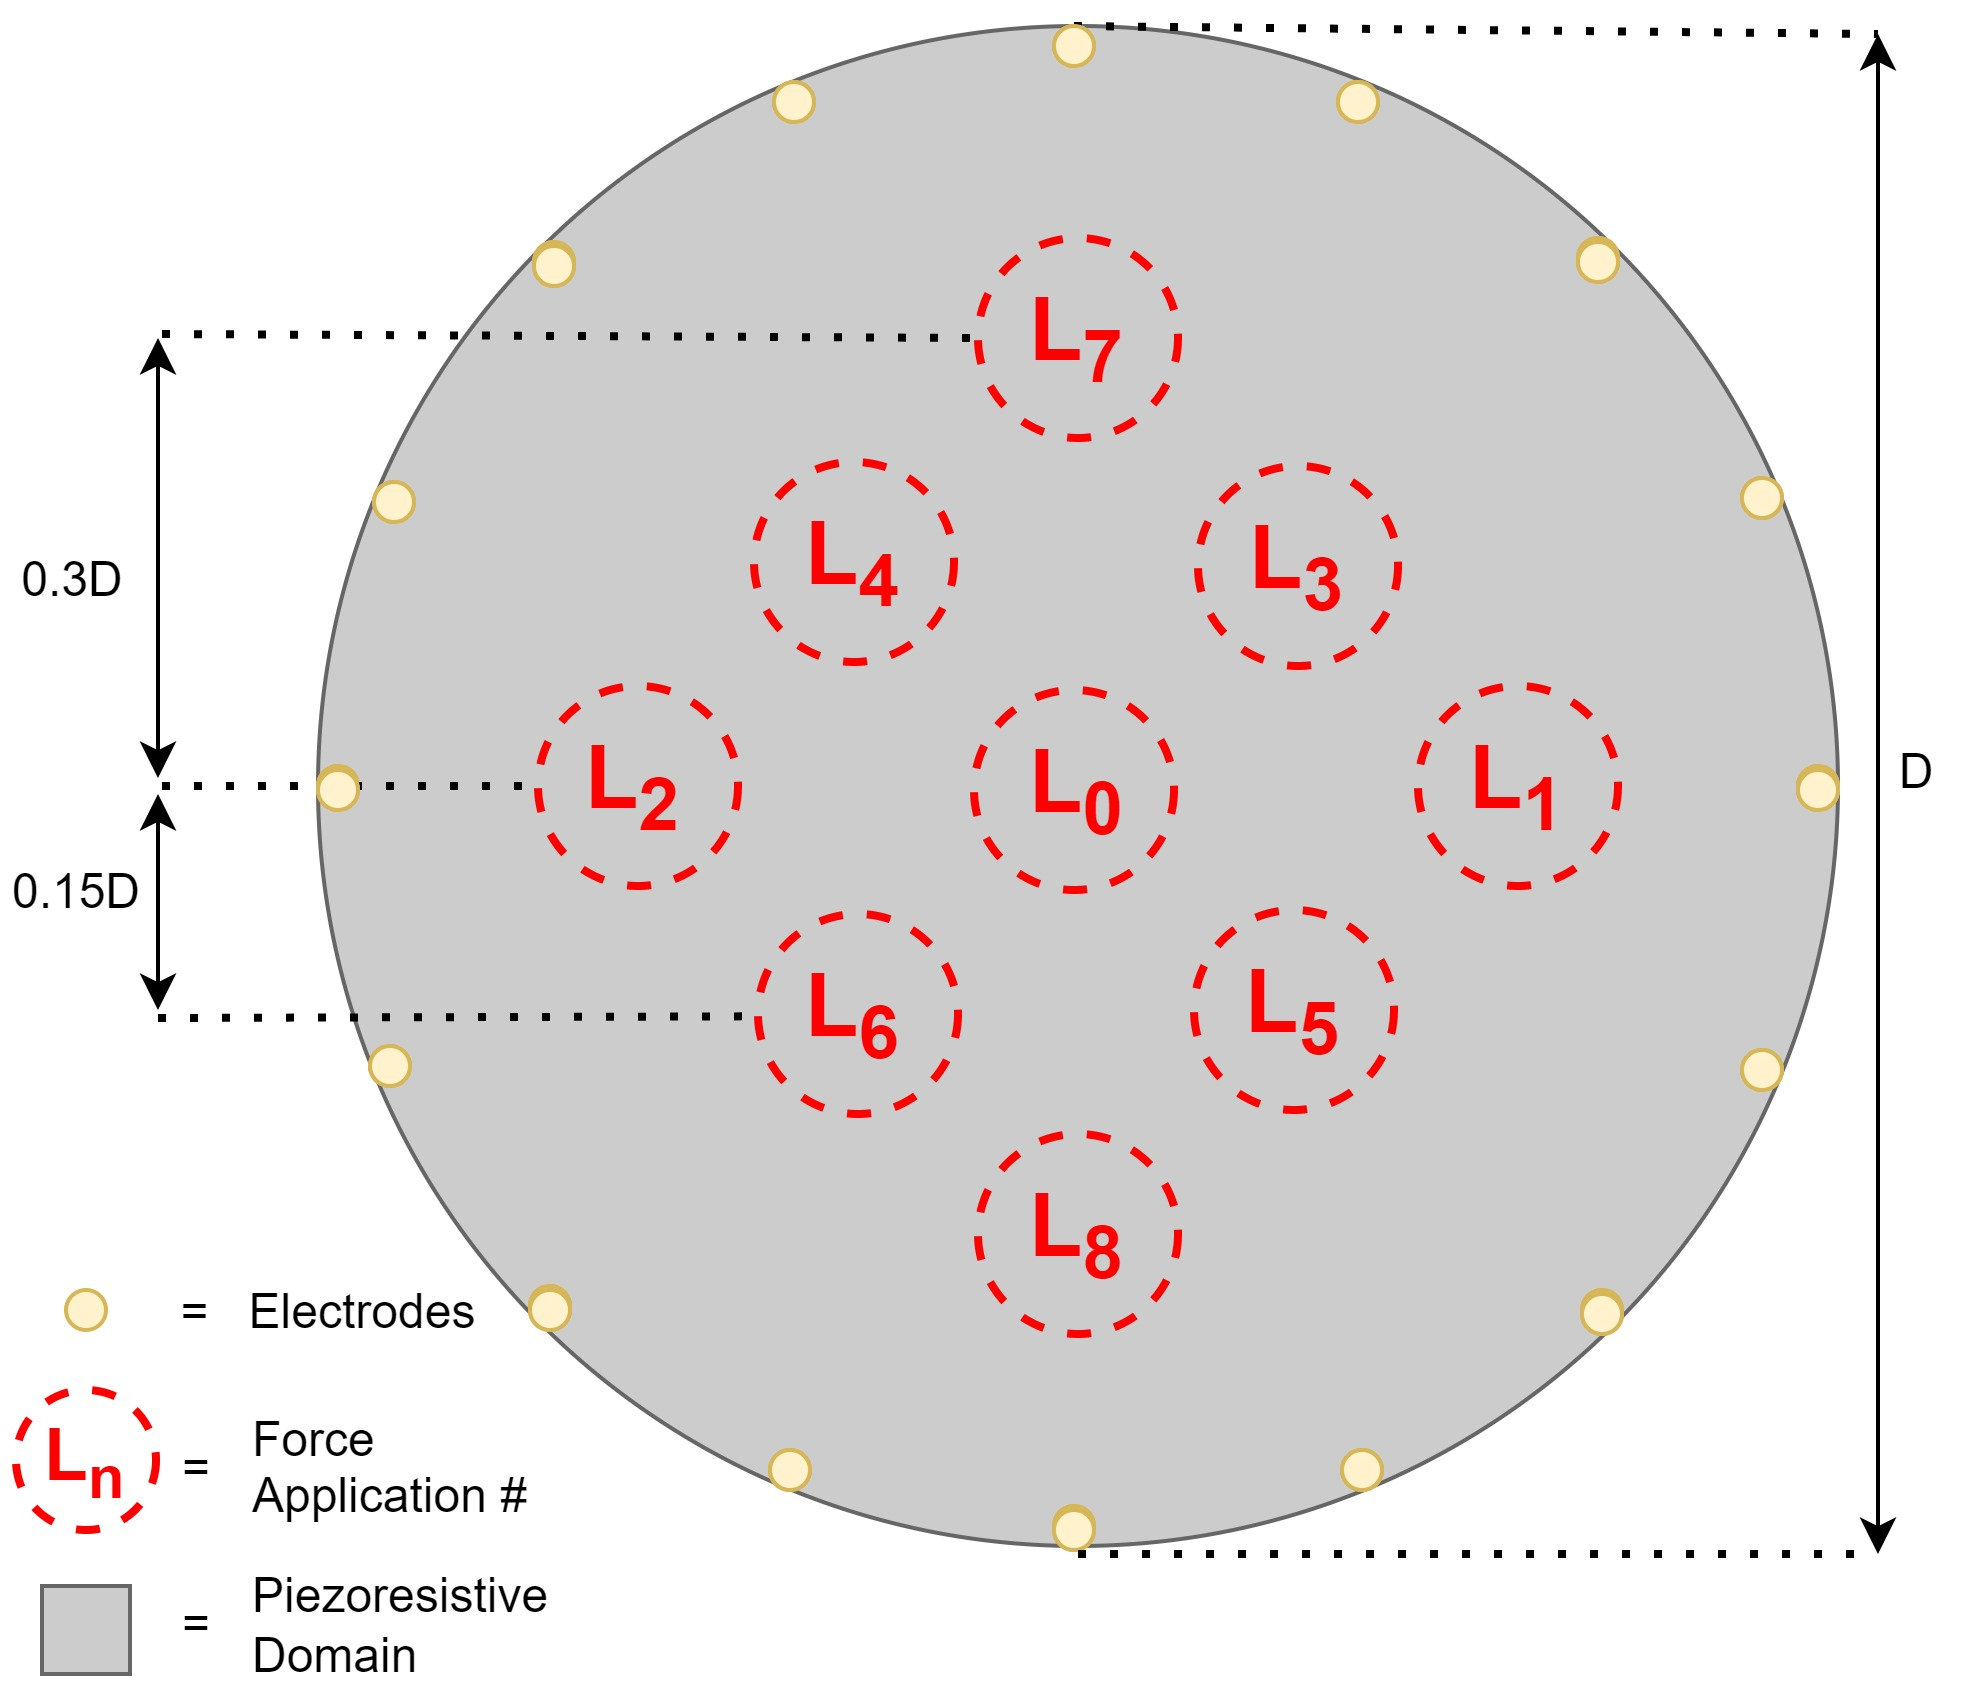
\includegraphics[width=8cm]{Figures/EIT_force_app_points_v3.11.jpg}
        \vspace{0.2cm}
		\caption{Load application areas used for compressive stress testing in order of application\cite{Ellingham2024} .}
		\label{fig:force_app_map}
	\end{figure}
	A Cartesian force applicator applied the loads with varying strains in the nine locations. Once the compliant electrodes had undergone the first load application tests, they were applied to each side of a DEA and tested again using the same sequence of nine loads. Compressive strains from 0 to 30\% of the electrode thickness in 5\% increments were applied to each of the load points using a flat circular 13 mm diameter force applicator. When applying the compressive strain to the compliant electrodes, a strain rate of of 16.67\%.s$^{-1}$ was used to minimise piezoresistive transient phenomena. After completing the load tests on individual compliant electrodes the compliant electrodes were attached to the DE surface. Next the load test was completed again with the DEA placed on a flat surface.
	\begin{figure}[H]Stre
		\centering
		\subfloat[$E_{CoM}$]{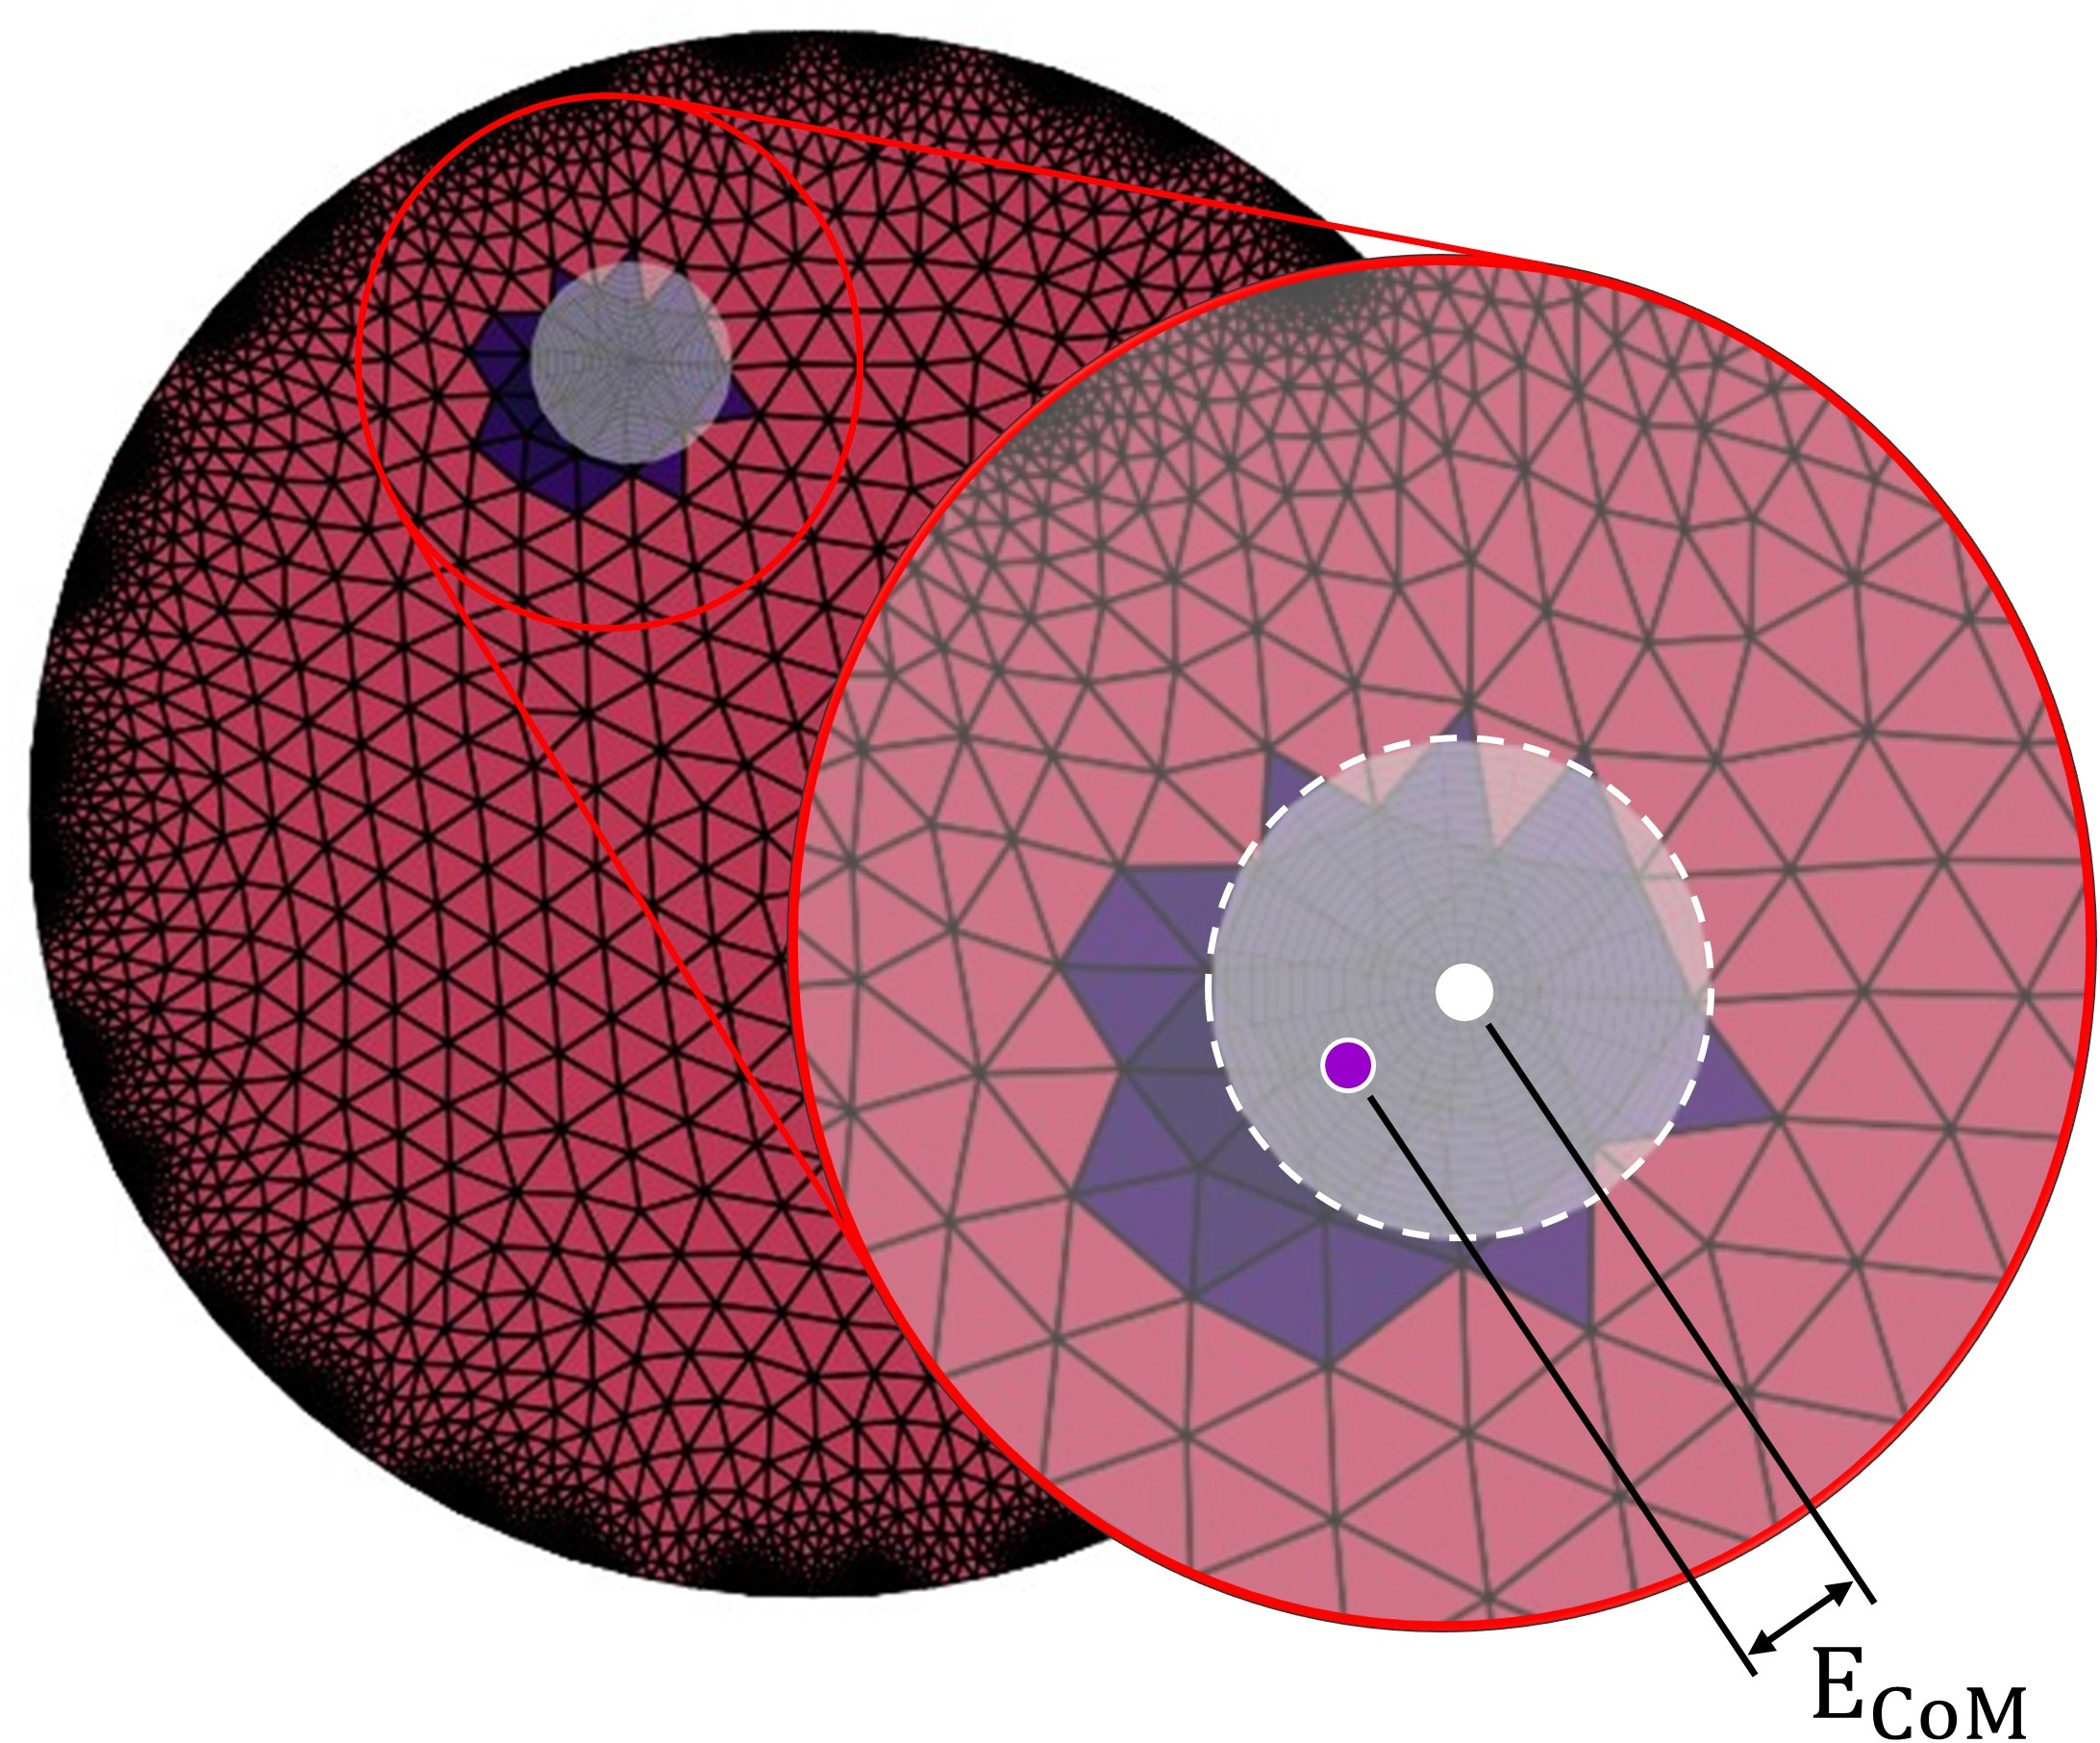
\includegraphics[width = 7cm]{Figures/eg_ecom_DEA2_EIT_CBSR_8p_1_9push_10strain_120s_1mA_1_frame800_th75.jpg}\label{subfig:eg_ecom}}
		\hspace{1cm}
		\subfloat[$S\!F$]{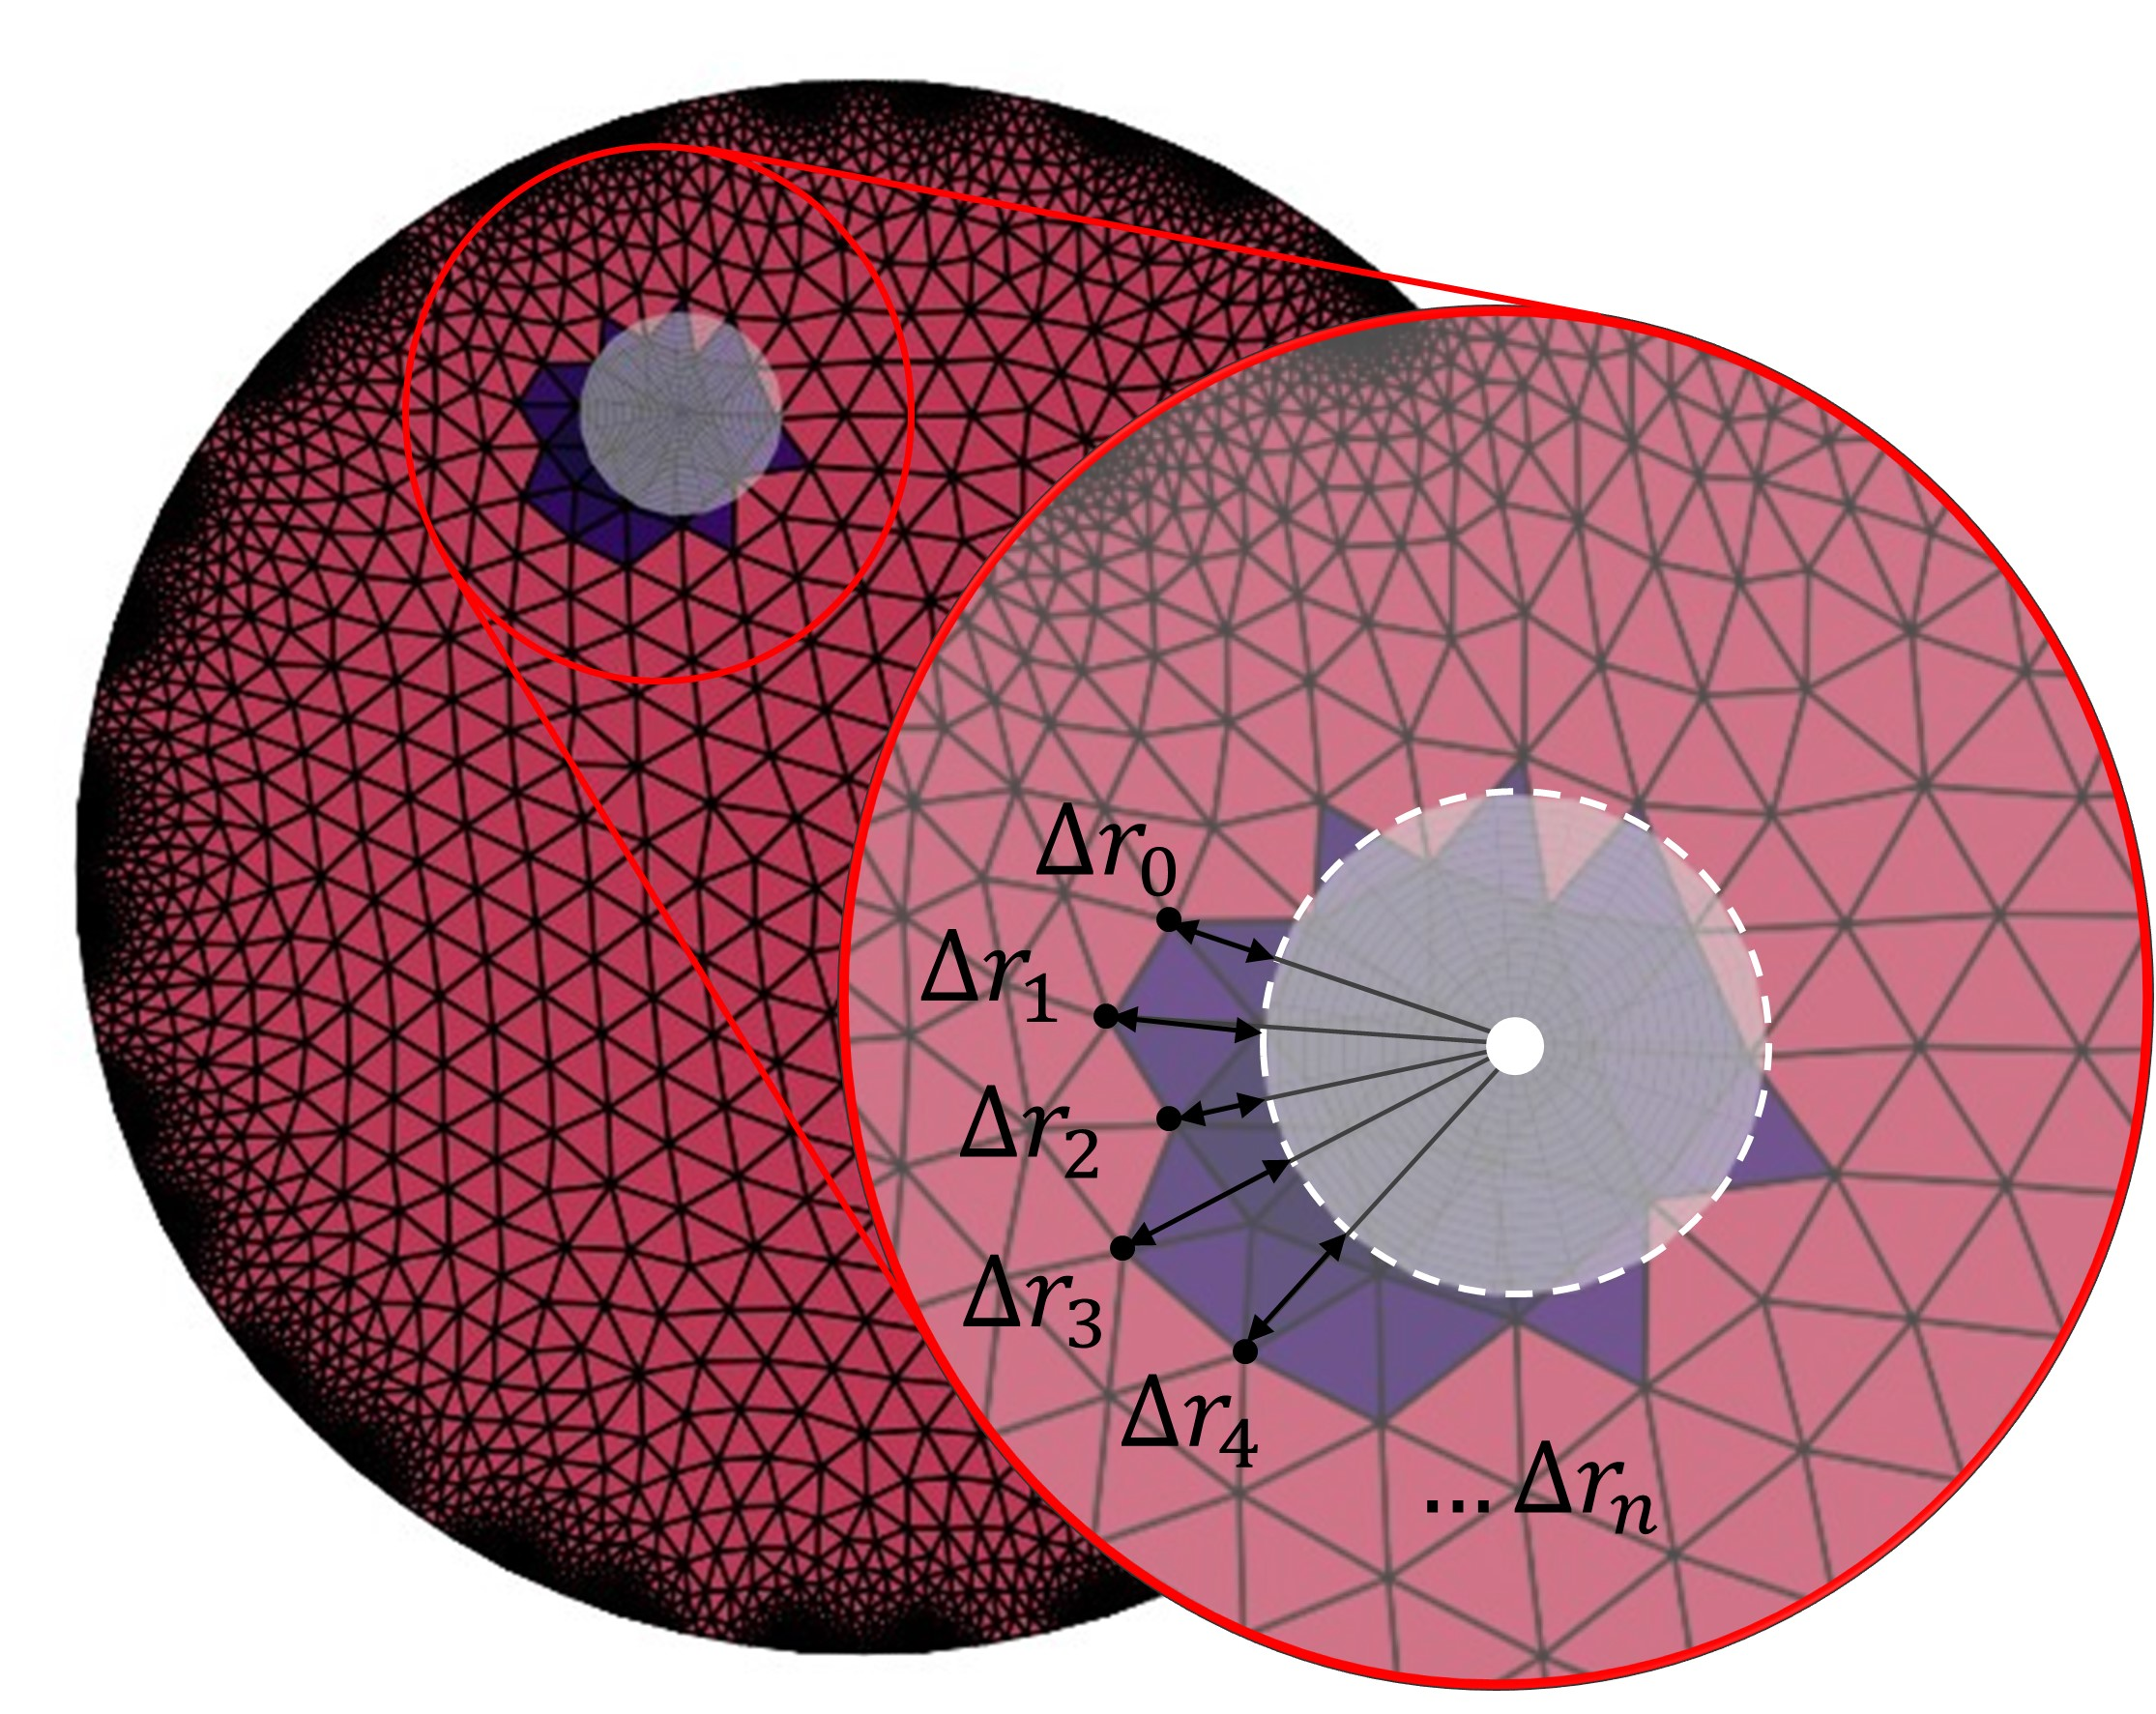
\includegraphics[width = 7cm]{Figures/eg_sf_DEA2_EIT_CBSR_8p_1_9push_10strain_120s_1mA_1_frame800_th75.jpg}\label{subfig:eg_sf}}
		\vspace{0.2cm}
		\caption{Spatial performance metrics used for determining the accuracy of a blob as a load area estimate.}
		\label{fig:eg_spatial_metrics}
	\end{figure}
    \begin{equation}
        S\!F = \left( \sum^i_n \Delta r_i^2 \right) / n
        \label{eqn:sf}
    \end{equation}
	After gathering all of the experimental data from applied loads, the data was used to generate EIT conductance images. To form blobs as estimates of the applied loads, post-processing was completed by applying an 85 \% threshold mask to the EIT image. These blob images were subsequently analysed using two spatial performance metrics, the centre-of-mass error, $E_{CoM}$, and the shape fit, $S\!F$, as exemplified in Figure \ref{fig:eg_spatial_metrics}. The $E_{CoM}$ values were determined by calculating the difference between the CoM of the actual load and the blob representing the load estimate. The $S\!F$ was determined by calculating the radial mean square error between all of the, $n$, perimetral nodes of the blob load estimate and the actual load circumference, as taken from the CoM of the actual load area.

 	To ensure the EIT domain reconstruction was geometrically accurate the circumferential electrodes were modelled in the meshing software to the same width as the real circumferential electrodes. However, the embedded depth of the circumferential electrode was not modelled. Due to the manual nature of the fabrication, significant error of up to 3 mm in the circumferential spacing of the rigid EIT electrodes was present, a factor which would be improved in future iterations.
	
	
	
	\section{RESULTS AND DISCUSSION} % 2 pages
	\label{sec:results_n_discu}
	A system was created that could both generate strain and map strain events using common DEA componentry with a circular DEA topology. The major limitations of integrating the two technologies were explored and quantified as a starting point for the further optimisation of such a device through the results given in this section.
 
	\subsection{Fabrication}
	\label{subsec:fab_results}
	Fabrication methods were successfully developed to create a range compliant electrode composites for successful DEA actuation and EIT-based pressure mapping. Prior to constructing the DEA, the compliant CBSR inter-electrode resistances, $R_{int}$, were measured  in a similar fashion to voltage shown in Figure \ref{fig:EIT_diagram} to ensure the sufficient conductivity and CB dispersion for DEA actuation and EIT-based sensing. The $R_{int}$ values between the adjacent circumferential electrodes for all samples was consistently $<$ 20 k$\Omega$, as shown in Table \ref{tab:NF_vals}. These $R_{int}$ values indicated a sufficiently low resistance for our electrical drive circuitry setup and indicates sufficiently homogeneous CB dispersion. Further validation to check the homogeneity of the whole domain could be done using other invasive or non-invasive methods such as a nail-bed resistance test and/or spectroscopic imaging. Inhomogeneity quantification at a scale smaller than that of the thickness of the material sample is important to obtain a higher SNR and hence $N\!F$ value.

    Stress-strain characterisation of DEs in literature clearly shows a hyperelastic softening effect between 50 to 400 \% strain for VHB film material, whereby the elastic modulus decreases to 40 - 70 kPa\cite{Liu2018} . This is significantly less than the assumed $\sim$ 142 kPa elastic modulus resulting from a 10 \% pre-stretch in this work. This hyperelastic region should be determined using both the DE and compliant electrode materials' hyperelastic regions to ensure the $K_{e\!f\!f}$ is minimised for maximal actuation strain, $S_{z_{de}}$. 
	% TODO: insert table for different average inter-electrode resistances for 0.5, 1, and 2 mm electrodes given in the EIT section
	% TOOD: Could gather data for the DE capacitance across all DEA samples. Why? This capacitance may be related to the rate of actuation due RC time constants of each thickness of compliant electrode.
	
	
	\subsection{DEA Validation}
	\label{subsec:dea_validation2}
	Before testing the piezoresistive compliant electrodes for both actuation and pressure mapping capability, the reference DEA was tested for its voltage actuation strain relationship. The theoretical actuation strain versus voltage was compared to the measured strain for the reference DEA shown in Figure \ref{subfig:ref_DEA}. The actuation strain data gathered is shown in \ref{fig:ref_DEA_results}. The range given was derived from substituting the range of $K$ and $\varepsilon_r$ parameters found in previous similar works\cite{Liu2018, Helal2018, Huang2023} into Equations \ref{eqn:DEA_stress} - \ref{eqn:DEA_strain_z_r}.
	\begin{figure}[H]
		\centering
		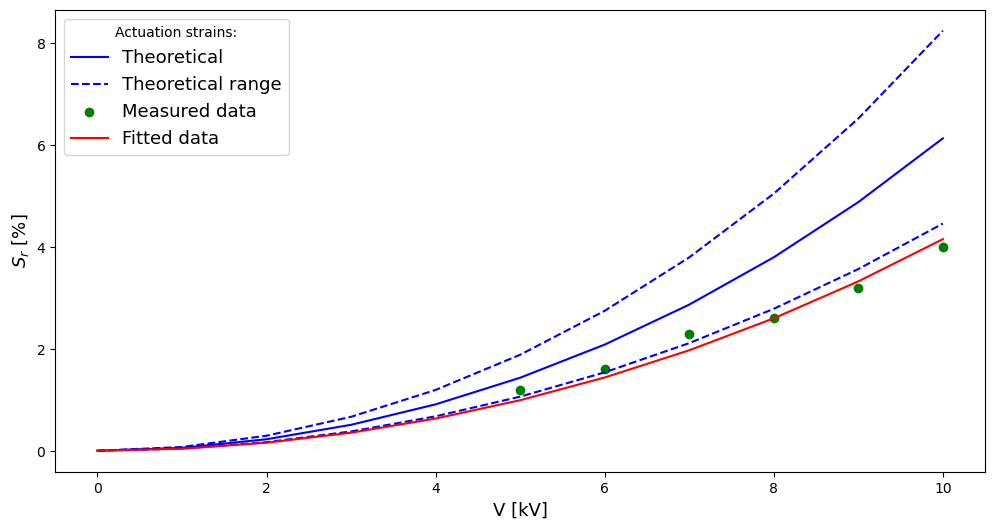
\includegraphics[width = 0.8\textwidth]{Figures/CB_vs_theory_range_vs_fitv2.png} % TODO: determine a range of K and perm_r values that put our experiment within the range given.
        \vspace{0.2cm}
		\caption{Comparing the measured CB reference DEA strain, the theoretical strain average and range, and the data fitted to Equation \ref{eqn:DEA_strain_z_r} by fitting either parameter $K$ or $\varepsilon_r$.}
		% \caption{Comparing the measured DEA strain, the theoretical strain given the assumed $K$ and $\varepsilon_r$ values, 142 kPa and 4.5 respectively, and the fitted curve using either assumed $K$ or $\varepsilon_r$ value and fitting the other. X* denotes the fitted parameter given our assumption of the other parameter is correct.}
		\label{fig:ref_DEA_results}
	\end{figure}
	Through actuation testing of different compliant electrodes applied to a DEA, models were fitted to the voltage-strain data gathered. The curve fit shown in Figure \ref{fig:ref_DEA_results} was found to have a linear set of solutions for $K$ and $\varepsilon_r$ with values similar to those limits of the material given characterisation determined in previous literature \cite{Carpi2003} .
	
	The CBSR compliant electrode experiments showed significantly smaller strains relative to the DEA with the CB powder compliant electrode as displayed in Figure \ref{fig:DEA_CBSR_thickness_results}. The effective mechanical impedance for the DEA with the CBSR compliant electrodes was significantly increased due to the relative thickness of the CBSR electrode and similar bulk modulus relative to the DE VHB material. Hence an effective bulk modulus, $K_{e\!f\!f}$, was calculated from fitting to the measured data, as a sum of the existing DE bulk modulus, $K$, and the effect of the compliant electrode's bulk modulus. $K_{e\!f\!f}$ is the a key characteristic of using thick compliant electrodes on a DEA that limits the actuation performance. When calculating $K_{e\!f\!f}$, $\varepsilon_r$ is assumed constant, as the effects of this different compliant electrode thickness on $\varepsilon_r$ is assumed relatively negligible. % TODO?: Insert citation showing that the $\varepsilon_r$ is less variable than K_eff (ideally by an order of magnitude!)
	\begin{figure}[H]
		\centering
		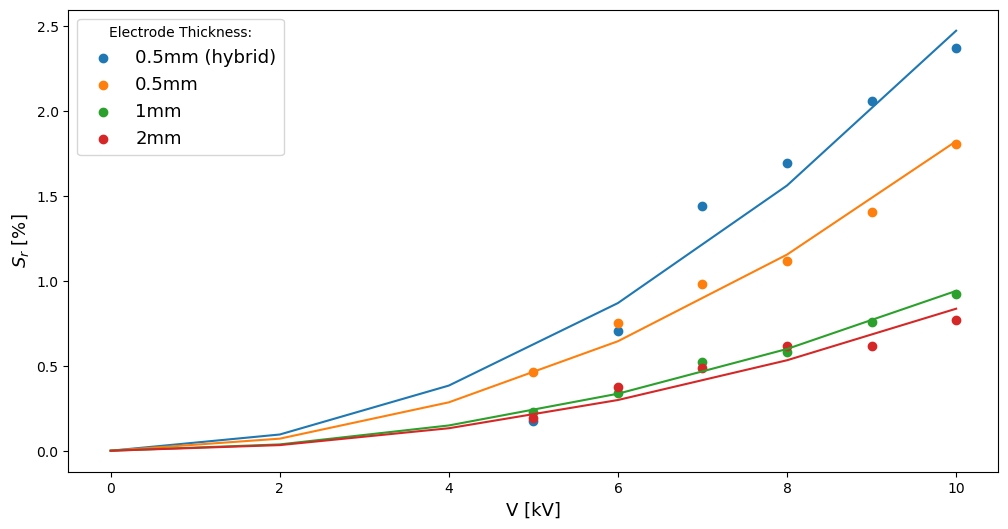
\includegraphics[width = 0.8\textwidth]{Figures/DEA_CBSR_thickness_strains_vs_fits_hyb.jpg}
        \vspace{0.2cm}
		\caption{Comparison of the voltage strain relationships between the 100 mm diameter compliant electrodes of various thicknesses, $z_{ce}$, used for the DEA.}
		\label{fig:DEA_CBSR_thickness_results}
	\end{figure}
	The effective bulk modulus impeding the actuation of the DE was calculated for each CBSR compliant electrode thickness by fitting to Equation \ref{eqn:DEA_strain_z_r} with the results displayed in Table \ref{tab:cbsr_bulk_mods}.
	\begin{table}[h!]
		\begin{center}
			\caption{Effective bulk modulus, $K_{e\!f\!f}$,  and coefficient of determination, $R^2$, for each fit of voltage-strain data for the CBSR compliant electrodes.}
			\vspace{0.5cm}
			\label{tab:cbsr_bulk_mods}
			\begin{tabular}{c|c|c} % TODO: R^2 OR determine stdev??
				$z_{ce}$ [mm] & $K_{e\!f\!f}$ [kPa] & $R^2$ \\
				\hline
				2 & 966 & 0.86\\
				1 & 860 & 0.99\\
				0.5 & 450 & 0.98 \\
				0.5 (hybrid) & 334 & 0.91\\
				% TODO?: add more hybridised results
			\end{tabular}
		\end{center}
	\end{table}
	To further enhance the actuation strain, $S_{z_{de}}$ of the DEA-EIT device, the compliant electrodes were hybridised such that one of the compliant electrodes was made from CB powder and the other from the CBSR composite. The hybridised results for the $K_{e\!f\!f}$ value are also given in Table \ref{tab:cbsr_bulk_mods}.

 	It is well known in literature and is intuitive that the mechanical characteristics of a DEA's compliant electrodes have a significant effect on the actuation performance \cite{Carpi2003, Zhang2020} . However, there has been a lack of empirical evidence and subsequent modelling on quantifying how much the thickness of a piezoresistive composite electrode affects actuation performance. This work provides empirical data to begin creating and validating models for thick electrode DEAs, as a step towards creating an objective function to optimise for a DEA for both actuation and sensing performance. 
	
	% TODO?: decide whether to include this analysis of the spider electrode styles... -->
	% After obtaining the results for the DEA actuation of various compliant electrodes thickness, it was hypothesised that altering the circumferential electrodes embedded in the boundary of the compliant electrodes would decrease $K_{e\!f\!f}$ and further enhance the actuation performance of the DEA. Hence a different configuration of the DEA was trialled which had different intermediary electrode material as an electrical connection between the compliant and the circumferential electrodes. The intermediary electrode materials tested were CB powder and a CB carbon grease mix.
	
	
	\subsection{EIT Validation}
	\label{subsec:eit_validation}
    EIT was used to map nine compressive loads applied throughout the material successfully. Validation of the EIT sensing method on the compliant electrodes was carried out for the three different electrode thickness, $z_{ce}$, values to see the differences the thickness may have on the pressure mapping characteristics' spatial performance. Figure \ref{fig:EIT_thickness_compare} exemplifies the difference in the conductance reconstructions for a load.
	\begin{figure}[H]
		\centering
		\subfloat[$z_{ce}$ = 0.5 mm]{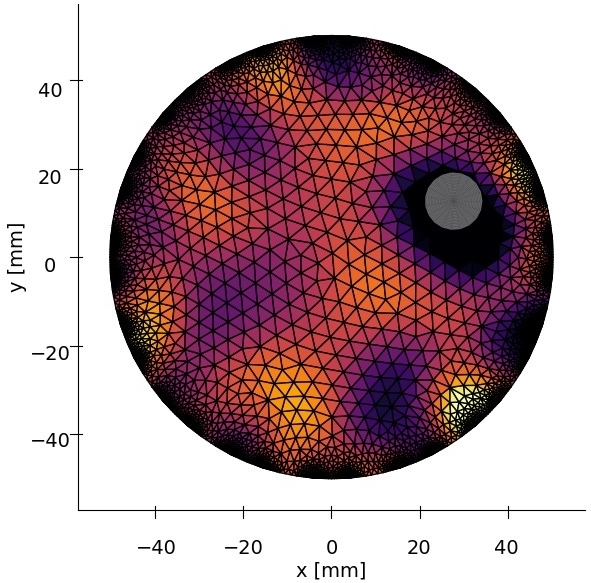
\includegraphics[width=5cm]{Figures/DEA.5_CBSR_8p_1_9push_15strain_120s_1mA_2_frame149.jpg}\label{subfig:DEA.5_strain15_L1}}
		\hspace{0.2cm}
		\subfloat[$z_{ce}$ = 1 mm]{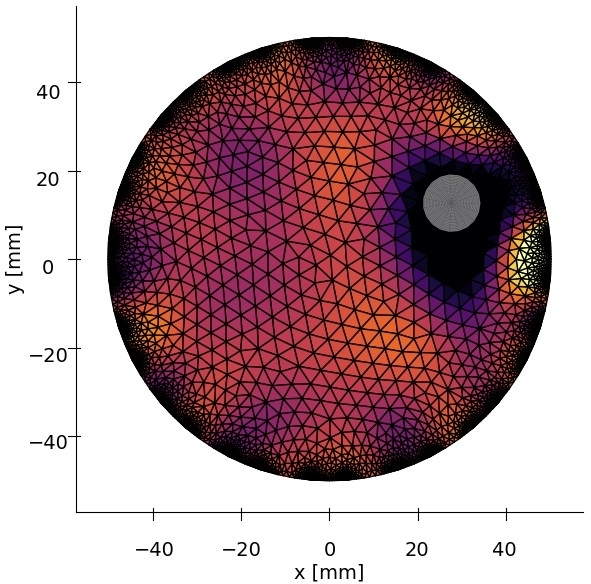
\includegraphics[width=5cm]{Figures/DEA1_CBSR_8p_1_9push_15strain_120s_1mA_2_frame134.jpg}\label{subfig:DEA1_strain15_L1}}
		\hspace{0.2cm}
		\subfloat[ $z_{ce}$ = 2 mm]{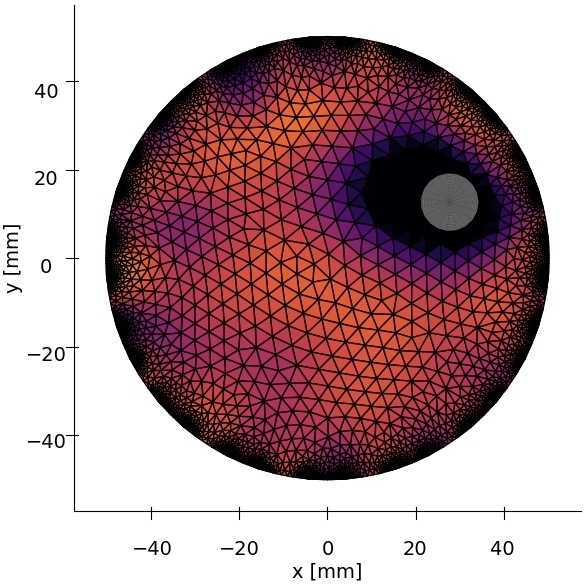
\includegraphics[width=5cm]{Figures/DEA2_CBSR_8p_1_9push_15strain_120s_1mA_2_frame162.jpg}\label{subfig:DEA2_strain15_L1}}
		\hspace{0.2cm}
		\subfloat[Scale]{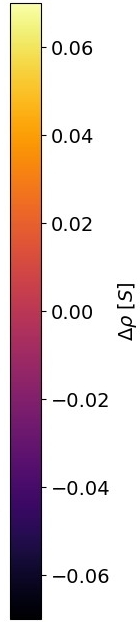
\includegraphics[width=1.2cm]{Figures/DEAX_CBSR_8p_1_9push_15strain_120s_1mA_2_cb.jpg}\label{subfig:DEAX_strain15_cbar}}
		\vspace{0.2cm}
		\caption{A 15\% strain compression at point $L_1$ applied to 100mm diameter compliant DEA electrodes of 3 compliant electrode thicknesses.}
		\label{fig:EIT_thickness_compare}
	\end{figure}
	A significant factor for determining the minimum pressure able to be detected is governed by the noise floor experienced when the domain is in a steady relaxed state. A metric used to quantify the noise floor is the noise figure, $N\!F$, which is commonly used in other applications\cite{Adler2009, Ellingham2024} of EIT.

 	A metric used to determine the minimum resistance change measured and hence pressure sensed is the $N\!F$ which can be seen analogously as a SNR. It was found that for increasing values of $z_{ce}$ the $N\!F$ values also increased.
 
    To quantify the domain homogeneity, the inter-electrode resistance, $\Bar{R}_{int}$ (of adjacent electrodes) data was gathered alongside the NF, as shown in Table \ref{tab:NF_vals}.
	\begin{table}[H]
		\centering
		\caption{Noise factor, $N\!F$, domain steady state noise, $\sigma_n$ and mean inter-electrode resistance, $\Bar{R}_{int}$, for each thickness of compliant DEA electrode used for EIT}
		\label{tab:NF_vals}
		\begin{tabular}{c|c|c|c}
			$z_{ce}$ [mm] & $N\!F$ & $\sigma_n$ [mS] & $\Bar{R}_{int}$ [k$\Omega$]\\
			\hline
			2 & 0.99 & 16.55 & 4.40 $\pm$ 0.69 \\
			1 & 0.98 & 27.48 & 7.72 $\pm$ 1.14\\
			0.5 & 0.96 & 38.86 & 9.91 $\pm$ 2.16\\
		\end{tabular}
	\end{table}
	To quantify the localisation performance of the loads applied to the DEA compliant electrode the centre-of-mass error, $E_{CoM}$, and shape fit, $S\!F$, of the sensing system were calculated. From three nine load experiments a set of mean $E_{CoM}$ is given in Table \ref{tab:spatial_metrics}. 

 % A polar histogram plot of the $E_{CoM}$ values from each frame from an experiment are displayed in Figures \ref{subfig:e_com_500um_dea} - \ref{subfig:e_com_1mm_dea}.
 
 % The vectorised format of the $E_{CoM}$ gave an indication of consistent biases that were present in the sample domains when compared across several repetitions of the same experiment. The vectorised $E_{CoM}$ values do not appear random and may instead be due to inhomogeneity. This data could be used in future in a calibration stage to determine how pressure sensed in particular regions may be spatially biased and preemptively corrected.

	% \begin{figure}[H]
	% 	\centering
 %  		\subfloat[$z_{ce}$ = 0.5 mm]{\includegraphics[width=5cm]{Figures/polar_ecom_DEA.5_CBSR_8p_1_9push_20strain_120s_1mA_1_simp.jpg}\label{subfig:e_com_500um_ce}}
	% 	\hspace{0.1cm}
	% 	\subfloat[$z_{ce}$ = 1 mm]{\includegraphics[width=5cm]{Figures/polar_ecom_DEA1_CBSR_8p_1_9push_20strain_120s_1mA_1_simp.jpg}\label{subfig:e_com_1mm_ce}}
	% 	\hspace{0.1cm}
	% 	\subfloat[$z_{ce}$ = 2 mm]{\includegraphics[width=5cm]{Figures/polar_ecom_DEA2_CBSR_8p_1_9push_20strain_120s_1mA_1_simp.jpg}\label{subfig:e_com_2mm_ce}}
	% 	\hspace{0.1cm}
	% 	\subfloat[Load locations]{\includegraphics[width=1.4cm]{Figures/polar_ecom_Lx_legend.jpg}\label{subfig:lx_legend_ce}}
	% 	\vspace{0.2cm}
	% 	\caption{Vectorised $E_{CoM}$ for the nine load experiment at 20\% compressive strain for each $z_{ce}$ value tested on individual DEA-EIT compliant electrode samples.}
	% 	\label{fig:polar_ecoms}
	% \end{figure}
	% \begin{figure}[H]
	% 	\centering
 %  		\subfloat[$z_{ce}$ = 0.5 mm]{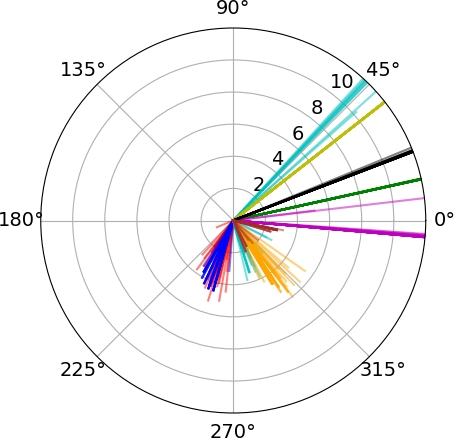
\includegraphics[width=5cm]{Figures/polar_ecom_DEA.5_EIT_CBSR_8p_1_9push_20strain_120s_1mA_1_simp.jpg}\label{subfig:e_com_500um_dea}}
	% 	\hspace{0.1cm}
	% 	\subfloat[$z_{ce}$ = 1 mm]{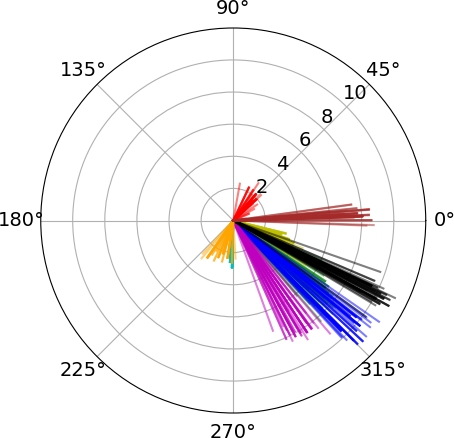
\includegraphics[width=5cm]{Figures/polar_ecom_DEA1_EIT_CBSR_8p_1_9push_20strain_120s_1mA_1_simp.jpg}\label{subfig:e_com_1mm_dea}}
	% 	\hspace{0.1cm}
	% 	\subfloat[$z_{ce}$ = 2 mm]{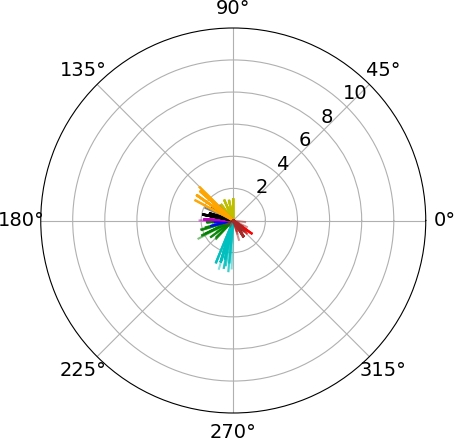
\includegraphics[width=5cm]{Figures/polar_ecom_DEA2_EIT_CBSR_8p_1_9push_20strain_120s_1mA_1_simp.jpg}\label{subfig:e_com_2mm_dea}}
	% 	\hspace{0.1cm}
	% 	\subfloat[Load locations]{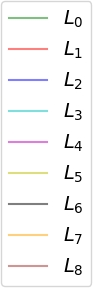
\includegraphics[width=1.4cm]{Figures/polar_ecom_DEA_EIT_Lx_legend.jpg}\label{subfig:lx_legend_dea}}
	% 	\vspace{0.2cm}
	% 	\caption{Vectorised $E_{CoM}$ for the nine load experiment at 20\% compressive strain for each $z_{ce}$ value tested on the DEA-EIT integrated samples.}
	% 	\label{fig:polar_ecoms}
	% \end{figure}
	Mean values for the spatial performance metrics, $E_{CoM}$ and $S\!F$, were gathered for each strain, each thickness, and at each load point. Spatial performance metric means from one nine load experiment are given in Table \ref{tab:spatial_metrics}. The $S\!F$ values are found using Equation \ref{eqn:sf}.
	\begin{table}[H]
		\centering
		\caption{Mean $E_{CoM}$ and $S\!F$ values ($\pm$ std) obtained for each DEA compliant electrode thickness at 20\% strains loads}
		\label{tab:spatial_metrics}
		\begin{tabular}{c|c|c}
			$z_{ce}$ [mm] & $\Bar{E}_{CoM}$ [mm] & $\Bar{S\!F}$ [mm$^2$] \\
			\hline
			2 & 4.99 $\pm$ 65.2 \% & 48.86 $\pm$ 7.86\\ % TODO: redo SF values!
			1 & 7.82 $\pm$ 90.4 \% & 49.32 $\pm$ 11.79\\
			0.5 & 21.03 $\pm$ 74.2 \% & 68.74 $\pm$ 31.18\\
		\end{tabular}
	\end{table}
	% \begin{table}[H]
	% 	\centering
	% 	\caption{Mean $E_{CoM}$ and $S\!F$ values ($\pm$ std) obtained for each DEA compliant electrode thickness at 20\% strains loads}
	% 	\label{tab:spatial_metrics}
	% 	\begin{tabular}{c|c|c}
	% 		$z_{ce}$ [mm] & $\Bar{E}_{CoM}$ [mm] & $\Bar{S\!F}$ [mm$^2$] \\
	% 		\hline
	% 		2 & 7.90 $\pm$ 0.73 & 46.03 $\pm$ 0.51\\ % TODO: redo SF values!
	% 		1 & 28.72 $\pm$ 3.36 & 36.93 $\pm$ 0.92\\
	% 		0.5 & 121.90 $\pm$ 24.84 & 81.92 $\pm$ 8.43\\
	% 	\end{tabular}
	% \end{table}
	% \begin{table}[H]
		%     \centering
		%     \caption{Mean shape fit, $S\!F$ ($\pm$ Std), values obtained for each DEA compliant electrode thickness at 20\% strains loads}
		%     \label{tab:spatial_metrics}
		%     \begin{tabular}{c|c|c|c}
			%         \multirow{ 2}{*}{$L_x$} & \multicolumn{3}{c}{$\Bar{S\!F}$  [mm$^2$] for $z_{ce}$:} \\
			%         & 0.5 mm & 1 mm & 2 mm \\
			%         \hline
			%         0 & 131.29 $\pm$ 6.18 & 18.40 $\pm$ 1.24 & 22.44 $\pm$ 1.15 \\
			%         1 & 45.18 $\pm$ 1.73 & 57.36 $\pm$ 1.42 & 54.22 $\pm$ 0.35 \\
			%         2 & 48.40 $\pm$ 1.91 & 29.11 $\pm$ 2.00 & 57.42 $\pm$ 0.39 \\
			%         3 & 74.22 $\pm$ 24.04 & 59.42 $\pm$ 0.48 & 62.26 $\pm$ 0.75 \\
			%         4 & 111.13 $\pm$ 15.09 & 46.81 $\pm$ 0.90 & 71.52 $\pm$ 0.42 \\
			%         5 & 132.32 $\pm$ 0.10 & 12.97 $\pm$ 0.28 & 11.81 $\pm$ 0.31 \\
			%         6 & 93.45 $\pm$ 24.76 & 3.01 $\pm$ 0.52 & 11.74 $\pm$ 0.32 \\
			%         7 & 101.13 $\pm$ 2.04 & 104.26 $\pm$ 1.39 & 122.76 $\pm$ 0.88 \\
			%         8 & 0.20 $\pm$ 0.03 & 0.99 $\pm$ 0.08 & 0.08 $\pm$ 0.01\\
			%     \end{tabular}
		% \end{table}
    % \subsection{Attached OR Detached Compliant DEA Electrodes EIT Validation}
    % TODO: determine whether attaching the CBSR to the DE had any significant effect on the sensing capability of the DEA.\\
    % TODO: determine whether the spider-like DEA topology seen in Figure \ref{subfig:DEA_EIT_multi} had any significant effect on the sensing capability of the DEA.


 	\subsection{Simultaneous Actuation and Mapping}
	This work has shown that using the same device for both actuation and pressure mapping shows promise and key learnings about how such a device can be further optimised have been elucidated. In future work, systems could be devised such that the sensing and actuation would be completed in real-time, so that applications requiring human-like manipulation can be realised from biomedical to agricultural processes. Another un-explored research avenue is the structural health monitoring of DEAs using EIT. It may also be possible to alter the system given in this work to map the location and size of any dielectric breakdown using EIT concurrently on each compliant electrode. This would allow for more technology to be developed around the self-healing of DEAs.
	
	
	\section{CONCLUSIONS}
	\label{sec:concs}
    This work set out to complete force mapping on the compliant electrode of a DEA using EIT and determine any limitations in the process. Three thicknesses of DEA with attached electrodes successfully showed actuation behaviour. Effective bulk moduli values were found to quantify the mechanical actuation impedance of each compliant electrode thickness used, ranging from 334 to 966 kPa. Force mapping was successful with decreasing degrees of mapping error with increasing compliant DEA electrode thickness. A mean centre-of-mass error of 7.9 $\pm$ 0.73 was found for the thickest used, 2 mm, compliant DEA electrode. The next steps for this research are to model the thick compliant DEA electrodes, complete a repeatability analysis of the pressure mapping performance metrics, and apply an inverse model to obtain reliable force estimates.